%************************************************
\chapter{Data sets}
\label{chp:data}
%************************************************

%========================================================================%
\section{GPS data}
%========================================================================%
\label{chp:data.sec:gpsdata}

%------------------------------------------------------------------------%
\subsection{Chicago Data}
%------------------------------------------------------------------------%
\label{chp:data.sec:gpsdata.sec:chicago}

Two data sets were used collected from 13 university shuttle busses serving the University of Illinois at Chicago campus \citep{chicago}. 

The data is sampled at 1 Hz, using commodity, low-cost SiRF-3 GPS receivers installed in 13 vehicles. Spatial resolution of this data is 0.000001 degrees latitude and longitude (less than 0.1m), offset by GPS noise with a standard deviation of 3.3m. Certain portions of the data contain significant noise (tens of meters) due to nearby high-rise buildings \citep{4inBiagioni}. We see this in two areas in particular.

The first data set was collected during 1 month, from the 1st of April to the 29th of April 2011. The trajectories cover an area of 3.92$\times$2.40 km. Further specifications can be seen in table \ref{tab:ch1m}.

%The Chicago dataset contains 889 GPS trajectories with a total length of 2869km (average: 3.22km and standard deviation: 894.28m) obtained from university shuttle buses covering an area of  (7km × 4.5km); the trajectories range from 100 to 363 position samples, with a sampling rate of 1s to 29s (average: 3.61s and standard deviation: 3.67s) \citep{localhomology}.


\begin{table}[H]
\centering
\caption{Specifications for Chicago 1 month data set.}
\label{tab:ch1m}
\begin{tabular}{cccccc}
      & \# traces & \# samples & \begin{tabular}[c]{@{}c@{}}sampling\\ rate {[}s{]}\end{tabular} & length {[}km{]} & \begin{tabular}[c]{@{}c@{}}duration\\ {[}d hh:mm:ss{]}\end{tabular} \\ \hline
total & 889.00     & 118'364.00    & n.a.                                                        & 2'869.00        & 4 22:02:08                                                      \\
min   & n.a.    & 100.00        & 1.00                                                           & 2.29        & 00:02:30                                                        \\
max   & n.a.    & 363.00        & 29.00                                                          & 8.84        & 00:20:19                                                        \\ 
mean  & n.a.    & 133.14    & 3.62                                                        & 3.22        & 00:07:58                                                        \\
std   & n.a.    & 36.72      & 3.68                                                        & 0.89       & 00:02:18                                                        \\

\hline
\end{tabular}
\end{table}

\begin{table}[H]
\centering
\caption{Specifications for Chicago 7 month data set.}
\label{tab:ch7m}
\begin{tabular}{cccccc}
      & \# traces & \# samples & \begin{tabular}[c]{@{}c@{}}sampling\\ rate {[}s{]}\end{tabular} & length {[}km{]} & \begin{tabular}[c]{@{}c@{}}duration\\ {[}d hh:mm:ss{]}\end{tabular} \\ \hline
total & 1'062.00            & 1'816'441.00  & n.a.                                                         & 44'215.25   & 115 19:34:27                                                    \\
min   & n.a.            & 1'000.00       & 1.00                                                            & 23.95       & 01:09:52                                                        \\
max   & n.a.            & 6'225.00       & 599.00                                                          & 148.37      & 09:22:32                                                        \\ 
mean  & n.a.            & 1'710.40    & 5.51                                                         & 41.63       & 02:37:02                                                        \\
std   & n.a.            & 768.93    & 19.82                                                        & 18.65       & 01:05:18                                                        \\
\hline
\end{tabular}
\end{table}


The second, larger, data set was collected over the course of 7 months, from the 1st of April to the 1st of November 2011. The trajectories cover and area of 3.89$\times$2.46 km. Further specifications can be seen in table \ref{tab:ch7m}. The raw GPS traces can further be seen in figure \ref{fig:data/chdata}.

\begin{figure}[H]%
 \centering
 \subfloat[\textit{Chicago 1 month data set.}]{{\includegraphics[width=\linewidth]{Figures/Data/raw_data_1m.pdf}\label{fig:data/ch1m} }}%   
 
 \subfloat[\textit{Chicago 7 month data set.}]{{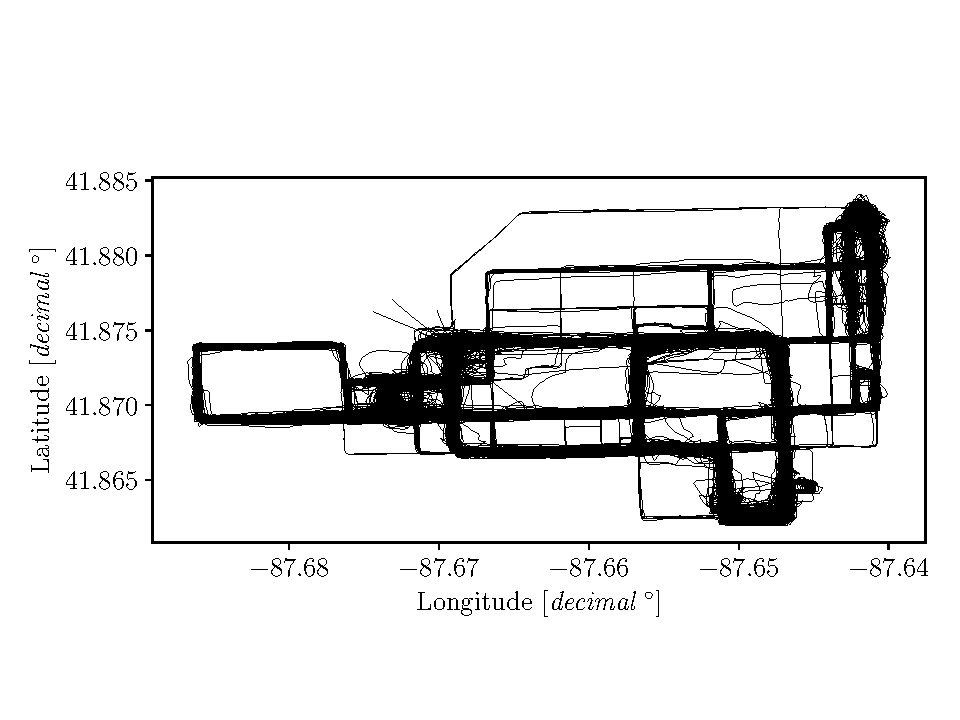
\includegraphics[width=\linewidth]{Figures/Data/raw_data_7m.pdf}\label{fig:data/ch7m} }}%
 \caption{Raw GPS traces plotted for the Chicago data sets.}%
 \label{fig:data/chdata}
\end{figure}


%------------------------------------------------------------------------%
\subsection{Data from Zenuity}
%------------------------------------------------------------------------%
%Non-smoothed and smoothed

The \textit{DriveMe} project, started by Volvo in 2013, was a first effort in investigating the possibilities and challenges with self-driving cars \citep{volvo}. The data that will be used, provided by Zenuity, was collected in 2016 from the 28th of June to the 13th of October. The data is sampled at 1Hz, using commodity SPA GPS receivers. The positional accuracy is in the order of 5--10 m. The trajectories cover an area of 16.3$\times$12.5 km. Further specifications can be seen in table \ref{tab:ch7m} and a visualisation of the raw traces in figure \ref{fig:data/dm}.

\begin{table}[H]
\centering
\caption{Specifications for the \textit{DriveMe} data set.}
\label{tab:data/dm}
\begin{tabular}{cccccc}
      & \# traces & \# samples & \begin{tabular}[c]{@{}c@{}}sampling\\ rate {[}s{]}\end{tabular} & length {[}km{]} & \begin{tabular}[c]{@{}c@{}}duration\\ {[}d hh:mm:ss{]}\end{tabular} \\ \hline
total & 2'512.00     & 124'578.00    & n.a.                                                        & 2'345.22     & 1 16:06:09                                                      \\

min   & n.a.     & 2.00          & 0.03                                                       & 0.01      & 00:00:00                                                        \\
max   & n.a.     & 62.00         & 59.10                                                        & 2.93        & 00:01:00                                                        \\
mean  & n.a.     & 49.59      & 1.18                                                        & 0.93        & 00:00:57                                                        \\
std   & n.a.     & 15.66      & 1.51                                                        & 0.52        & 00:00:07                                                        \\
\hline
\end{tabular}
\end{table}

\textbf{står det tydligt att min, max, mean osv är för varje trip file? och vad en trip file är? att det är en trajecgtory/trace}


\begin{figure}[H]
    \centering
    \includegraphics[width=\linewidth]{Figures/Data/raw_data_drive_me.pdf}
    \caption{Raw GPS traces plotted for the \textit{DriveMe} data set.}
    \label{fig:data/dm}
\end{figure}


\textbf{LÄGG TILL ATHEN!!!!!!!}


\newpage
%------------------------------------------------------------------------%
\subsection{Bounding boxes}
%------------------------------------------------------------------------%

The coordinates for the bounding box that each data set covers is reported in table \ref{tab:data/bbox}.

\begin{table}[H]
\centering
\caption{Bounding boxes for each data set.}
\label{tab:data/bbox}
\begin{tabular}{ccccc}
                           &     & Chicago 1 month & Chicago 7 month & DriveMe   \\ \hline
\multirow{2}{*}{latitude [decimal °]}  & min & 41.862  & 41.862  & 57.623 \\
                           & max & 41.884  & 41.884  & 57.736 \\
\multirow{2}{*}{longitude [decimal °]} & min & -87.687 & -87.687 & 11.842 \\
                           & max & -87.640 & -87.640 & 12.038 \\
area [km$^2$] & &  9.420 & 9.570 & 203.864                           \\ \hline
\end{tabular}
\end{table}

% \subsection{Simulated data}
% Sumo, \ac{OSM}

%------------------------------------------------------------------------%
\subsection{Accuracy of \ac{GPS} data}
%------------------------------------------------------------------------%

The purpose of the thesis was to evaluate road network change detection methods when only consumer grade, or low precision, \ac{GPS} data is available, meaning 5--10 meter precision. More accurate high precision \ac{GPS} data, such as RTK with centimetre precision, exists but is more expensive. Therefore, it is desirable to find a feasible alternative to the expensive high precision \ac{GPS} data. By exploring a map generation methodology robust to noise, we hope to find a feasible alternative using low precision \ac{GPS} data. 

\newpage
%========================================================================%
\section{OSM and OSMnx - Python for Street Networks}
\label{chp:data.sec:osm}
%========================================================================%

\ac{OSM} is an open source project for maps \citep{osm}. They aim to create a free digital map of the world. This is done by having volunteering participants collecting data in a central database. It is a concept similar to the ones of open source software development projects and is sometimes referred to as \ac{VGI} \citep{haklay}. In this project the \ac{OSM} was used as ground truth.

Furthermore, the Python package \textit{OSMnx} was used which allows you to download, visualise, project and construct street networks \citep{osmnx}. Since the earth is spherical, or rather slightly squeezed, one needs to project the map. For this the \textit{OSMnx} package was used. The map was saved as a .graphml-file which is a .xml-format. To further handle the .graphml-file in Python a Python package called \textit{pygraphml} was used to parse the data and obtain a graph representation of the road network.

We select bounding box for the area of interest, meaning where the \ac{GPS} data has been collected. For information of this see table \ref{tab:data/bbox}. Using this bounding box we retrieve the corresponding \ac{OSM} in the region. 

%------------------------------------------------------------------------%
\subsection{Extracting ground truth}
%------------------------------------------------------------------------%
\label{chp:data.sec:osm.sec:gt}

We ``verified'' an \ac{OSM} the following way. Since no information is available on where the vehicles actually travelled we have no real ground truth. Instead, based on where trajectories were observed to travel for each data set we manually extracted roads and discarded those that seemingly were not travelled on. This is an estimation of the ground truth, since we know that the \ac{GPS} data contained a lot of noise and that actual travel paths could be different from what is observed. However, for our purpose this estimation was assumed to be good enough. Ground truth was extracted for the Chicago 1 month and 7 month data sets and the result is seen in figure \ref{fig:data/osmdata}.

For the 1 month data set one trace travelled on a motor way. This road was disregarded, as we did not include motor ways when generating the \ac{OSM} for the Chicago data set and the busses in the 7 month data set were further not observed to travel here. 

\begin{figure}[H]%
 \centering
 \subfloat[\textit{\textit{Chicago 1 month data set.}}]{{\includegraphics[width=\linewidth]{Figures/Data/chicago_osm_1m.png}\label{fig:data/osm1m} }}% 
 
 \subfloat[\textit{Chicago 7 month data set.}]{{\includegraphics[width=\linewidth]{Figures/Data/chicago_osm_7m.png}\label{fig:data/osm7m} }}%
 \caption{Verified \ac{OSM} for the Chicago data sets.}%
 
 \label{fig:data/osmdata}
\end{figure}



\newpage
%========================================================================%
\section{Project data}
%========================================================================%

The earth is spherical or rather slightly squeezed. Since it is easier to handle a two-dimensional plane rather than a three-dimensional room one needs to project the map. To do this there are different geodetic systems that describes the earth as a ellipsoid. The global standard is called WGS 84 which is tied to an international system ITRF. In Sweden SWEREF 99 is primarily used which also is connected to ITRF. Differences between the different ITRF-based systems are only a couple of decimetres (The main difference between the two is that SWEREF 99 takes continental drift into accont which WGS 84 does not.)\citep{lant1}. In table \ref{tab:geodetic} the properties of the two ellipsoids are presented. They are represented by their semi-major axis, $a$, and inverse flattening, $1/f$. The inverse flattening is calculated by the ellipsoids semi-major axis, $a$, and semi-minor axis, $b$, as

\begin{equation}
    f = \frac{a-b}{a}.
\end{equation}

In figure \ref{fig:data/earth} we can see an illustration of the earth as an ellipsoid, described by its semi-major axis, $a$, and semi-minor axis, $b$ \citep{lant2}. 

\begin{table}[H]
\centering
\caption{Specifications of the ellipsoids of the geodetic systems \citep{lant2}\citep{lant3}.}
\label{tab:geodetic}
\begin{tabular}{lll}
                        & SWEREF 99     & WGS 84        \\ \hline
Semi-major axis, $a$ (m)  & 6378137.0     & 6378137.0     \\
Inverse flattening, $1/f$ & 298.257222101 & 298.257223563 \\ \hline
\end{tabular}
\end{table}


\begin{figure}[H]
    \centering
    \includegraphics[width=6cm]{Figures/Data/earth.png}
    \caption{The earth as an ellipsoid, described by its semi-major axis, $a$, and semi-minor axis, $b$ \citep{lant2}.}
    \label{fig:data/earth}
\end{figure}


